\documentclass[12pt]{article}
\usepackage{graphicx}
\usepackage{subcaption}
\usepackage[]{mcode}
\usepackage{mwe}
\usepackage{amsmath}
\usepackage[T1]{fontenc}
%\usepackage{lingmacros}
%\usepackage{tree-dvips}
%\usepackage{blindtext}
%\usepackage[utf8]{inputenc}

\renewcommand{\thesubsection}{\thesection.\alph{subsection}}

\begin{document}

\title{CMSC 460 - HW3}
\author{Gudjon Einar Magnusson}

\maketitle

\section{} %3.3

\subsection{}

Figure \ref{fig_interp_plot} shows the interpolated value of $x$ and $y$ using each of the interpolation methods.

\begin{figure}
    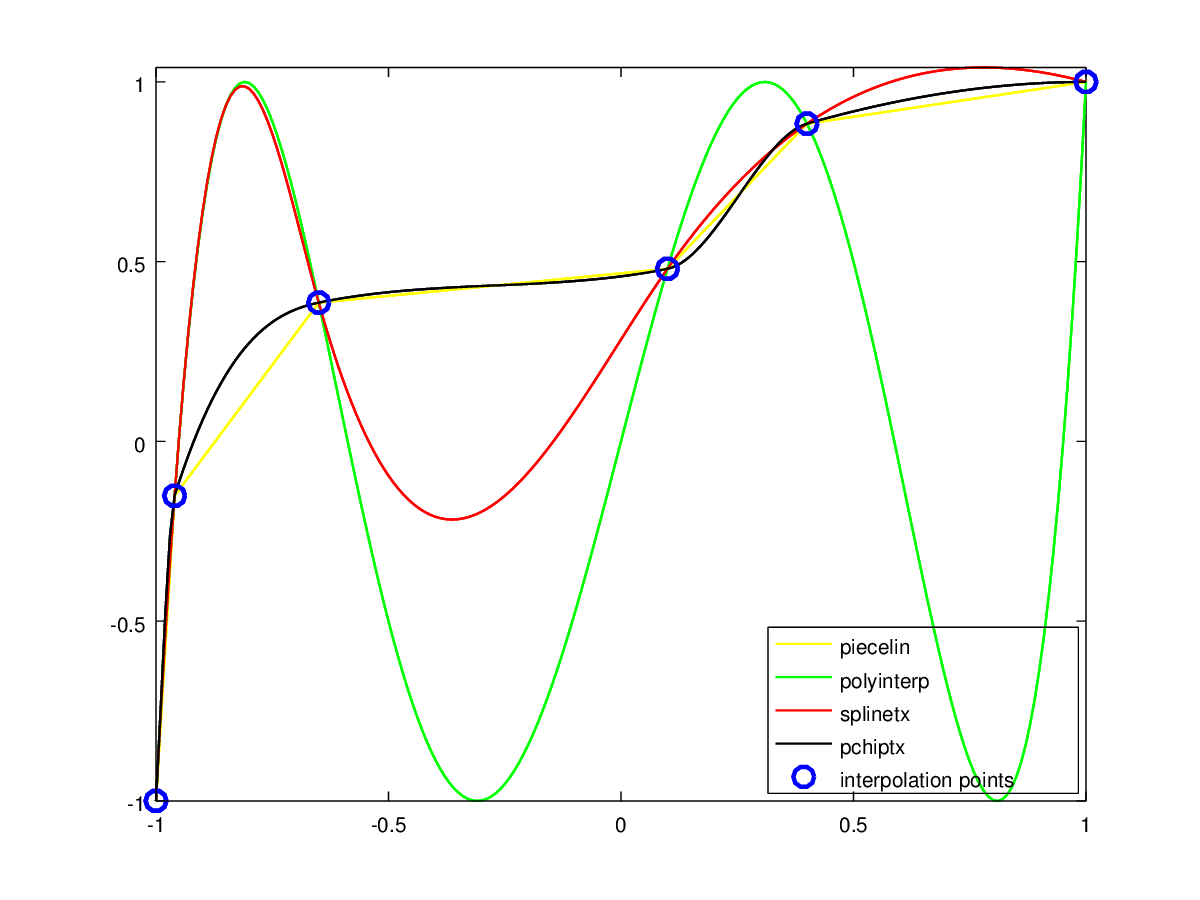
\includegraphics[width=0.6\linewidth]{interp_plot}
    \centering
    \caption{4 different ways to interpolate between 6 points}
    \label{fig_interp_plot}
\end{figure}

\subsection{}

For each of the interpolation methods I evaluated the function at $x = -0.3$.
\begin{description}
    \item[piecelin] \hfill \\
    $p(-0.3) = 0.42996$
    \item[polyinterp] \hfill \\
    $p(-0.3) = -0.999$
    \item[splinetx] \hfill \\
    $p(-0.3) = -0.1957$
    \item[pchiptx] \hfill \\
    $p(-0.3) = 0.43218$
\end{description}

In this case I prefer the result of \textit{pchiptx} and \textit{piecelin}. Its intuitively between the values at the surrounding points. Its makes minimal assumptions about the shape of the function.

\subsection{}

By using \textit{polyfit} and testing a few different degrees I found the coefficients $0,5,0,-20,0,16$. The polynomial is $p(x) = 0+5x+0-20x^3+0+16x^5$. Figure \ref{fig_px} shows a plot of $p(x)$.

Turns out \textit{polyinterp} provided the best interpolation.

\begin{figure}
    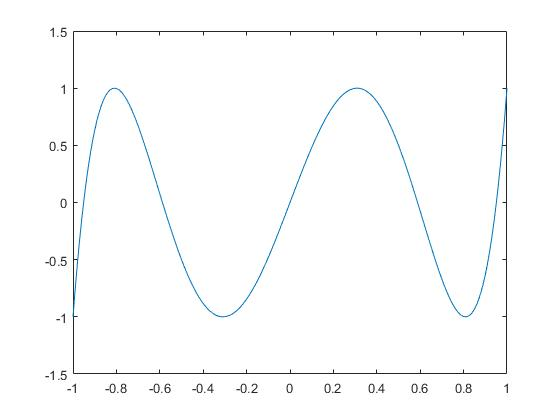
\includegraphics[width=0.6\linewidth]{poly}
    \centering
    \caption{$p(x) = 0+5x+0-20x^3+0+16x^5$}
    \label{fig_px}
\end{figure}

\section{} %3.4

Figure \ref{fig_hand} shows my hand plotted using two different methods. I prefer the one plotted using \textit{splinetx}, it looks much smoother. The one plotted using \textit{pchiptx} looks jagged.

Figure 3.11 in the book looks like it was plotted with \textit{splinetx}.

\begin{figure}[t!]
    \begin{subfigure}[t]{0.5\textwidth}
        \centering
        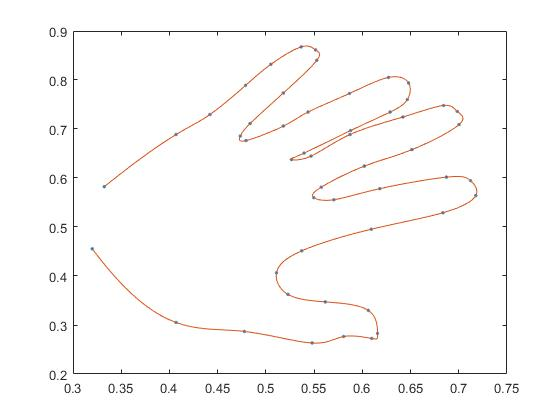
\includegraphics[width=\linewidth]{hand1}
        \caption{My hand plotted with \textit{splinetx}}
        \label{fig_hand1}
    \end{subfigure}
    \begin{subfigure}[t]{0.5\textwidth}
        \centering
        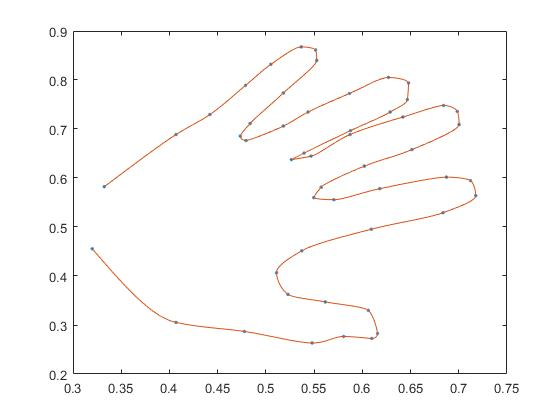
\includegraphics[width=\linewidth]{hand2}
        \caption{My hand plotted with \textit{pchiptx}}
        \label{fig_hand2}
    \end{subfigure}
    \caption{My hand plotted using 53 points}
    \label{fig_hand}
\end{figure}

\section{} %3.7

Suppose that $p(x)$ and $q(x)$ are two polynomials of degree less than $n$ that agree on $n$ points. That implies that there are $n$ distinct values $x_1, x_2, \dots , x_n$ such that $p(x_i) - q(x_i) = 0$. A polynomial of degree $n$ can have at most $n$ zeros unless it is the zero polynomial. Since $p - q$ has greater number of zeros than the degree of $p$ and $q$ it follows that the difference between $p$ and $q$ is $0$, therefore $p = q$.

\end{document}